\documentclass[10pt,portuguese,]{article}
\usepackage{lmodern}
\usepackage{amssymb,amsmath}
\usepackage{ifxetex,ifluatex}
\usepackage{fixltx2e} % provides \textsubscript
\ifnum 0\ifxetex 1\fi\ifluatex 1\fi=0 % if pdftex
  \usepackage[T1]{fontenc}
  \usepackage[utf8]{inputenc}
\else % if luatex or xelatex
  \ifxetex
    \usepackage{mathspec}
  \else
    \usepackage{fontspec}
  \fi
  \defaultfontfeatures{Ligatures=TeX,Scale=MatchLowercase}
\fi
% use upquote if available, for straight quotes in verbatim environments
\IfFileExists{upquote.sty}{\usepackage{upquote}}{}
% use microtype if available
\IfFileExists{microtype.sty}{%
\usepackage{microtype}
\UseMicrotypeSet[protrusion]{basicmath} % disable protrusion for tt fonts
}{}
\usepackage[textwidth=18cm,textheight=24cm]{geometry}
\usepackage{hyperref}
\hypersetup{unicode=true,
            pdfborder={0 0 0},
            breaklinks=true}
\urlstyle{same}  % don't use monospace font for urls
\ifnum 0\ifxetex 1\fi\ifluatex 1\fi=0 % if pdftex
  \usepackage[shorthands=off,main=portuguese]{babel}
\else
  \usepackage{polyglossia}
  \setmainlanguage[]{portuguese}
\fi
\usepackage{graphicx,grffile}
\makeatletter
\def\maxwidth{\ifdim\Gin@nat@width>\linewidth\linewidth\else\Gin@nat@width\fi}
\def\maxheight{\ifdim\Gin@nat@height>\textheight\textheight\else\Gin@nat@height\fi}
\makeatother
% Scale images if necessary, so that they will not overflow the page
% margins by default, and it is still possible to overwrite the defaults
% using explicit options in \includegraphics[width, height, ...]{}
\setkeys{Gin}{width=\maxwidth,height=\maxheight,keepaspectratio}
\IfFileExists{parskip.sty}{%
\usepackage{parskip}
}{% else
\setlength{\parindent}{0pt}
\setlength{\parskip}{6pt plus 2pt minus 1pt}
}
\setlength{\emergencystretch}{3em}  % prevent overfull lines
\providecommand{\tightlist}{%
  \setlength{\itemsep}{0pt}\setlength{\parskip}{0pt}}
\setcounter{secnumdepth}{5}
% Redefines (sub)paragraphs to behave more like sections
\ifx\paragraph\undefined\else
\let\oldparagraph\paragraph
\renewcommand{\paragraph}[1]{\oldparagraph{#1}\mbox{}}
\fi
\ifx\subparagraph\undefined\else
\let\oldsubparagraph\subparagraph
\renewcommand{\subparagraph}[1]{\oldsubparagraph{#1}\mbox{}}
\fi

%%% Use protect on footnotes to avoid problems with footnotes in titles
\let\rmarkdownfootnote\footnote%
\def\footnote{\protect\rmarkdownfootnote}

%%% Change title format to be more compact
\usepackage{titling}

% Create subtitle command for use in maketitle
\newcommand{\subtitle}[1]{
  \posttitle{
    \begin{center}\large#1\end{center}
    }
}

\setlength{\droptitle}{-2em}
  \title{}
  \pretitle{\vspace{\droptitle}}
  \posttitle{}
  \author{}
  \preauthor{}\postauthor{}
  \date{}
  \predate{}\postdate{}

\usepackage{booktabs}
\usepackage{longtable}
\usepackage{array}
\usepackage{multirow}
\usepackage[table]{xcolor}
\usepackage{wrapfig}
\usepackage{float}
\usepackage{colortbl}
\usepackage{pdflscape}
\usepackage{tabu}
\usepackage{threeparttable}

\usepackage{setspace}
\usepackage{indentfirst}
\usepackage[utf8]{inputenc}
\usepackage{mathptmx}
\usepackage{enumerate}
\usepackage{url}
\usepackage{float}
\usepackage{lipsum}
\usepackage{multirow}
\usepackage{booktabs}
\usepackage{longtable}
\usepackage{subcaption}

\begin{document}

\begin{titlepage}
\thispagestyle{empty}
\begin{center}
\begin{center}
\begin{minipage}[s]{1.75cm}
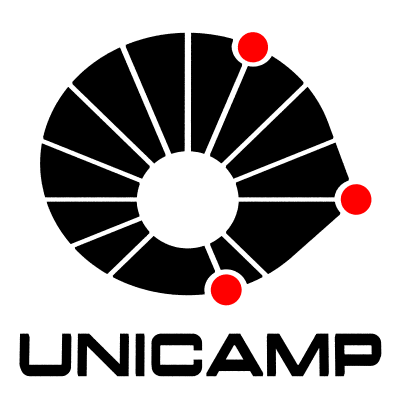
\includegraphics[width=40pt,height=45pt]{logoUnicamp.png} 
\end{minipage}\begin{minipage}[s]{11.25cm}\noindent
{\begin{center} {\Large Universidade Estadual de Campinas}\\
{Instituto de Matemática, Estatística e Computação Científica}\\
{\sc Departamento de Estatística}
\end{center}}
\end{minipage}
\begin{minipage}[s]{0.5cm}

\includegraphics[width=40pt,height=45pt]{logoimecc.png}
\end{minipage}
\end{center}
\end{center}
\vspace{3cm}
\font\fontGrande=cmcsc10 scaled 2500
\font\pessoal=cmr9 scaled 2500

\begin{center}
\vspace*{3.5cm}
{\rule[0 ex]{16cm}{0.05cm}}
{\huge \sc Trabalho - Parte 2 \\[8pt]
Relatório - Questão 1}
{\rule[0 ex]{16cm}{0.05cm}}
\end{center}

\begin{center}

\normalsize \vspace{8mm}


\vspace{4cm}

{\sc  Eliane Ramos de Siqueira  RA:155233} \\
{\sc  Guilherme Pazian  RA:160323}\\
{\sc  Henrique Capatto  RA:146406}\\
{\sc  Murilo Salgado Razoli  RA:150987}

\vspace{0.2cm}

Disciplina: {\bf ME731 - Análise Multivariada}\\
Professor: {\bf Caio Lucidius Naberezny Azevedo}
\vspace{1cm}

{\footnotesize{Campinas - SP \\ 24 de Novembro de 2017}}
\end{center}
\end{titlepage}

\setlength{\parindent}{3em} \doublespacing

\begin{enumerate}
\def\labelenumi{\arabic{enumi}.}
\tightlist
\item
  Introdução \vspace{0.5cm} \doublespacing
  O Salmão é um peixe cujo mercado tem uma importância significante para
  economia, como podemos ver na Tabela 1. A fronteira do Canadá com o
  Alasca é uma importante área de pesca de salmão, exerce forte
  influência na escassez ou abundância deste peixe (em um próximo ciclo
  reprodutivo) no local de reprodução. Existem basicamente dois tipos de
  Salmão nessa região: um que nasce no Alasca e outro que nasce no
  Canadá. Devido a proximidade, um salmão nascido no Alasca, pode acabar
  sendo pescado no mar por um pescador do Canadá e vice versa. Os
  salmões nascem em água doce mas migram para o mar e retornam,
  posteriormente, para o local onde nasceram, para fins de reprodução.
  Por isso, caso grande parte da população de salmão nascida em um local
  específico for pescado, ocorre uma diminuição na quantidade de salmãos
  que conseguirão se reproduzir neste local, gerando escassez destes
  peixes.
\end{enumerate}

Os pescadores do Alasca eram conhecidos por interceptar grandes
quantidades de salmão canadense, deixando os canadenses com menos
oportunidade de interceptar salmão originário do Alasca. Este fato gerou
alguns conflitos entre Estados Unidos e Canadá, tanto que em 1985 estes
países fizeram um tratado para pesca de salmão do Oceano Pacífico
(\emph{Pacific Salmon Treaty}), proibindo a pesca de salmão do tipo que
nasce no Canadá por pescadores norte americanos e do tipo que nasce no
Alasca por pescadores canadenses. Portanto, para facilitar o seguimento
do tratado, é imprescindível conseguir diferenciar os tipos de salmão
por sua região de origem. Mais informações sobre esse conflito na
referência 1 da bibliografia.

Neste relatório, pretende-se criar uma regra de classificação, visando
descomplicar a identificação da origem dos salmões pescados. O banco de
dados utilizado contém duas variáveis intituladas como DGAD e DGM
(diâmetro da guelra (em mm) na fase de água doce e diâmetro da guelra
(em mm) na fase no mar respectivamente) medidas em 50 salmões
provenientes do Alasca e em 50 salmões provenientes do Canadá, assim
como o gênero de cada peixe. Neste relatório, nos referiremos a origem
dos salmõesindistintamente como Região, localidade e/ou grupo.

Todas as análises foram realizadas com o suporte dos softwares \emph{R}
versão 3.4.2 e \emph{RStudio} versão 1.1.383.

Foi considerado um nível de significância de 5\% para tomada de decisões
quanto aos resultados dos testes estatísticos aqui apresentados.

\vspace{0.5cm}

\begin{table}[!h]
\centering
\caption{Informações sobre pesca de Salmão no ano de 2015 para Alasca (veja referência 2) e para Canadá ( veja referência 3)}
\bgroup
\def\arraystretch{1.0}
\begin{tabular}{lcc}
\toprule
\multicolumn{1}{l}{Origem} & \multicolumn{1}{l}{Toneladas} & \multicolumn{1}{l}{Mil Dólares (EUA)} \\ \midrule
\hline
Alasca                     & 120280                        & 494783                                \\
Canadá                     & 6534                          & 14168          \\ \bottomrule
   \hline
\end{tabular}
\egroup
\end{table}

\newpage

\begin{enumerate}
\def\labelenumi{\arabic{enumi}.}
\setcounter{enumi}{1}
\tightlist
\item
  Análise Descritiva
\end{enumerate}

\vspace{0.5cm}

A Tabela 2, apresenta algumas medidas resumo para as variáveis DGAD e
DGM separadas por região (Alasca e Canadá). É possível notar que as
média amostral para a variável DGAD é maior no Canadá, enquanto para a
variável DGM ocorre o oposto. Podemos notar também que os desvios padrão
para a variável DGM é consideravelmente diferente entre o Canadá e o
Alasca, já para a variável DGAD essa diferença é bem menor.

\vspace{0.5cm}

\vspace{0.5cm}

\begin{table}[ht]
\centering
\caption{Medidas Resumo das variáveis por região}
\bgroup
\def\arraystretch{1.0}
\begin{tabular}{rlllllllll}
  \toprule
 & Região & n & Media & Variancia & Desvio Padrao & CV(\%) & Minimo & Mediana & Maximo \\ \midrule
  \hline
\multirow{2}{*}{DGAD} & Alasca & 50 & 98,38 & 260,608 & 16,143 & 16,409 & 53 & 99 & 131 \\ 
   & Canadá & 50 & 137,46 & 326,09 & 18,058 & 13,137 & 90 & 140 & 179 \\ \midrule
\multirow{2}{*}{DGM} & Alasca & 50 & 429,66 & 1399,086 & 37,404 & 8,706 & 355 & 427,5 & 511 \\ 
   & Canadá & 50 & 366,62 & 893,261 & 29,887 & 8,152 & 301 & 369,5 & 438 \\ \bottomrule
   \hline
\end{tabular}
\egroup
\end{table}

A partir da Figura 1, que consta o gráfico de dispersão entre as
variáveis separadas por Região (Alasca e Canadá), podemos observar que
os peixes do Canadá tendem a ter um diâmetro (em mm) da guelra durante a
fase de água doce maior que os peixes do Alasca e durante a fase no Mar
tendem a ter um diâmetro menor (em mm). Se olharmos separadamente os
dois grupos, vemos que existe uma correlação levemente positiva de valor
0,25 entre os peixes do Canadá, e levemente negativa de valor -0,31 para
os peixes do Alasca. Vale ressaltar que se considerarmos ambos os
Grupos, parecer haver uma correlação negativa entre as variáveis.

\vspace{0.5cm}

\begin{figure}[!h]

{\centering 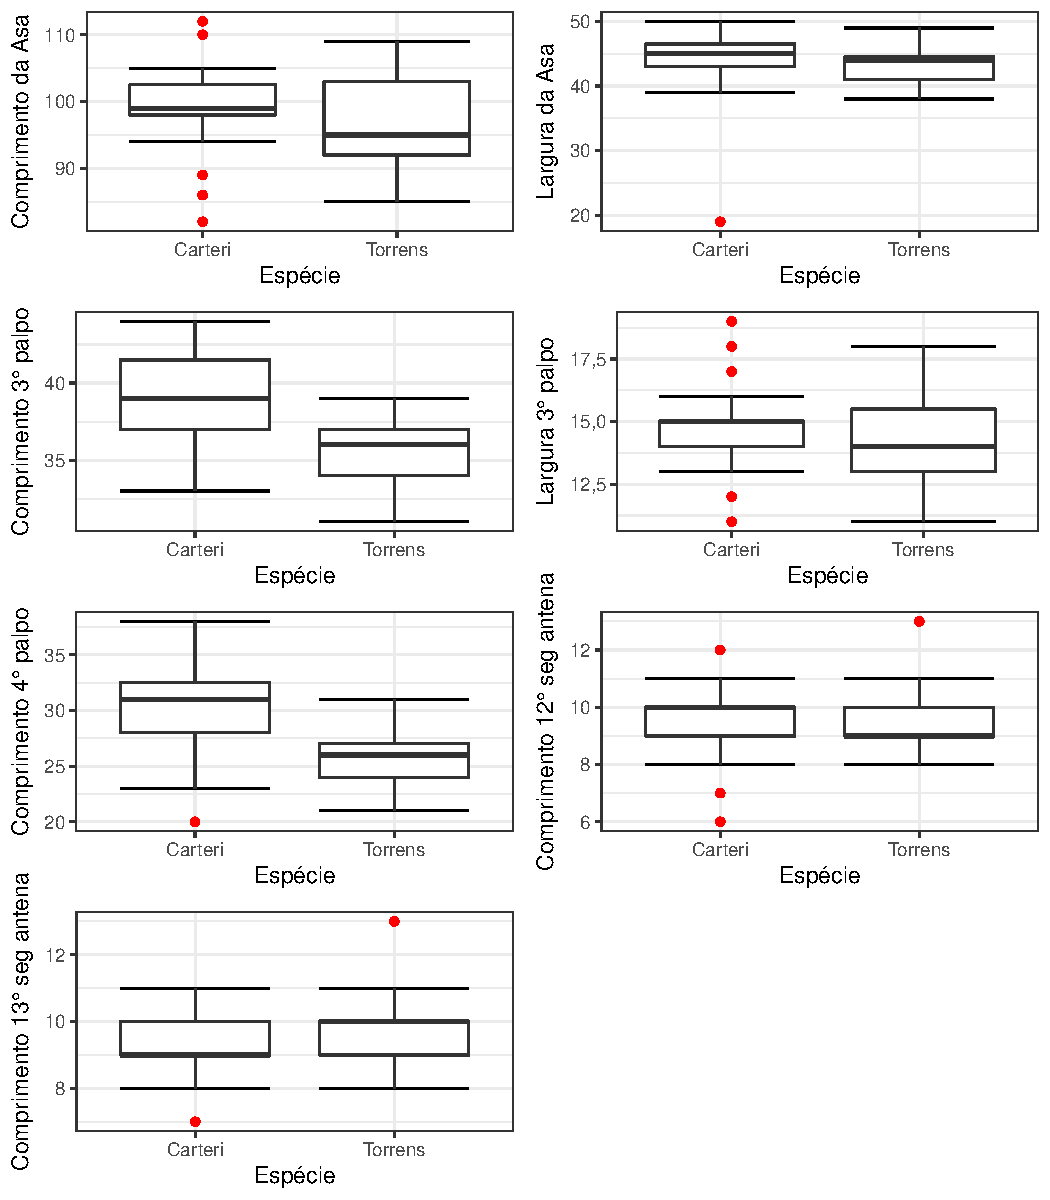
\includegraphics{RELATORIO_FINAL_FORMATADO_files/figure-latex/unnamed-chunk-10-1} 

}

\caption{Gráfico de dispersão entre os diâmetros da guelra de salmões em água doce e no mar}\label{fig:unnamed-chunk-10}
\end{figure}

\vspace{0.5cm}

Na Figura 2 notamos que o diâmetro da guelra é menor na água doce para
os peixes de ambos os grupos, o que constatamos também na distribuição
de densidade na Figura 3 e é reforçado nos valores das medidas centrais,
como a da média e mediana, na Tabela 2. Estes resultados são esperados
devido a natureza dos dados, pois as medidas em água doce foram obtidas
na fase inicial da vida dos peixes e as medições obtidas no mar
aconteceram na maturidade destes salmões.

Podemos observar também nos box-plot, que o diâmetro das guelras para o
salmão do Canadá é consideravelmente maior do que os do Alasca. Durante
a fase no mar, ocorre o contrário. Para ambas as variáveis (DGAD, DGM) é
possível notar uma sobreposição em boa parte da distribuições
apresentadas na Figura 3. As distribuições parecem ser levemente
assimétricas, mais evidente para o diâmetro da guelra no mar dos peixes
do Canadá, e menos evidente para diâmetro da guelra na água doce dos
salmões do Alasca.

\vspace{0.5cm}

\begin{figure}[!h]

{\centering 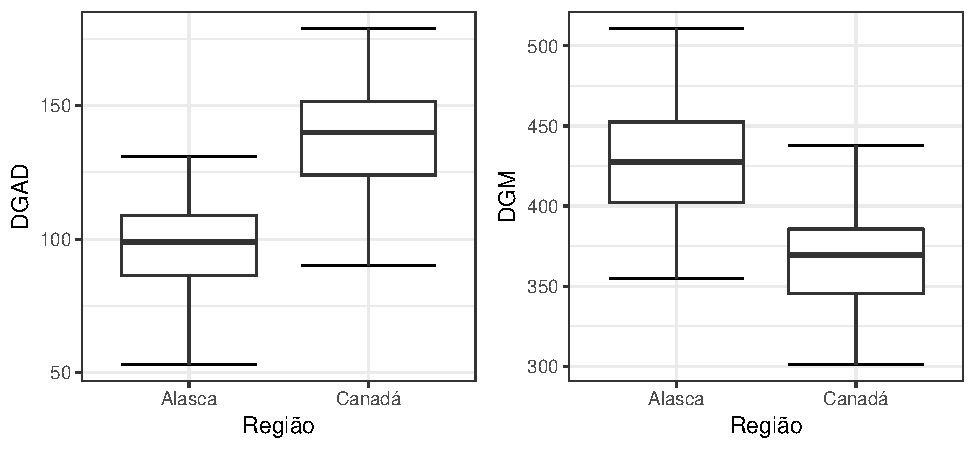
\includegraphics{RELATORIO_FINAL_FORMATADO_files/figure-latex/unnamed-chunk-11-1} 

}

\caption{Boxplots por grupo}\label{fig:unnamed-chunk-11}
\end{figure}

\vspace{0.5cm}

\begin{figure}[!h]

{\centering 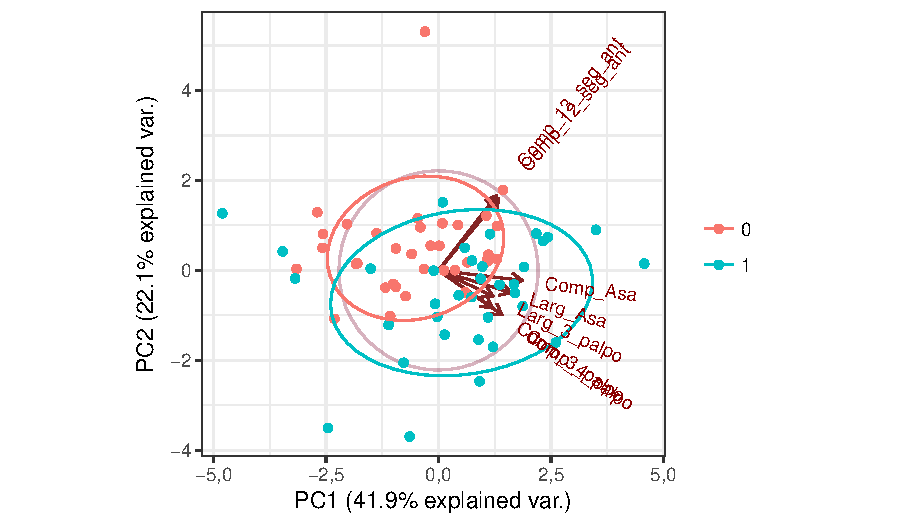
\includegraphics{RELATORIO_FINAL_FORMATADO_files/figure-latex/unnamed-chunk-12-1} 

}

\caption{Distribuição estimada por grupo}\label{fig:unnamed-chunk-12}
\end{figure}

Podemos observar na Figura 4 que para cada variável DGAD e DGM foi
realizado um gráfico de quantil-quantil para cada Grupo (Canadá e
Alasca). Vemos que para o diâmetro da guelra na fase em água doce de
peixes do Alasca, os pontos se comportaram de maneira razoavelmente
aleatória em torno da linha de referência, não apresentando sinais
evidentes de tendência. Os outros três gráficos, apresentam uma certa
sistematização no comportamento dos dados em torno da linha de
referência, evidenciando uma certa tendência, embora pareça ser menos
contundente, e configurando um ponto contra a suposição de normalidade
dos dados\textgreater{} Porém não seria irrazoável supor normalidade
para as variáveis neste caso dada a fraca intensidade desta tendência.

\vspace{0.5cm}

\begin{figure}[!h]

{\centering 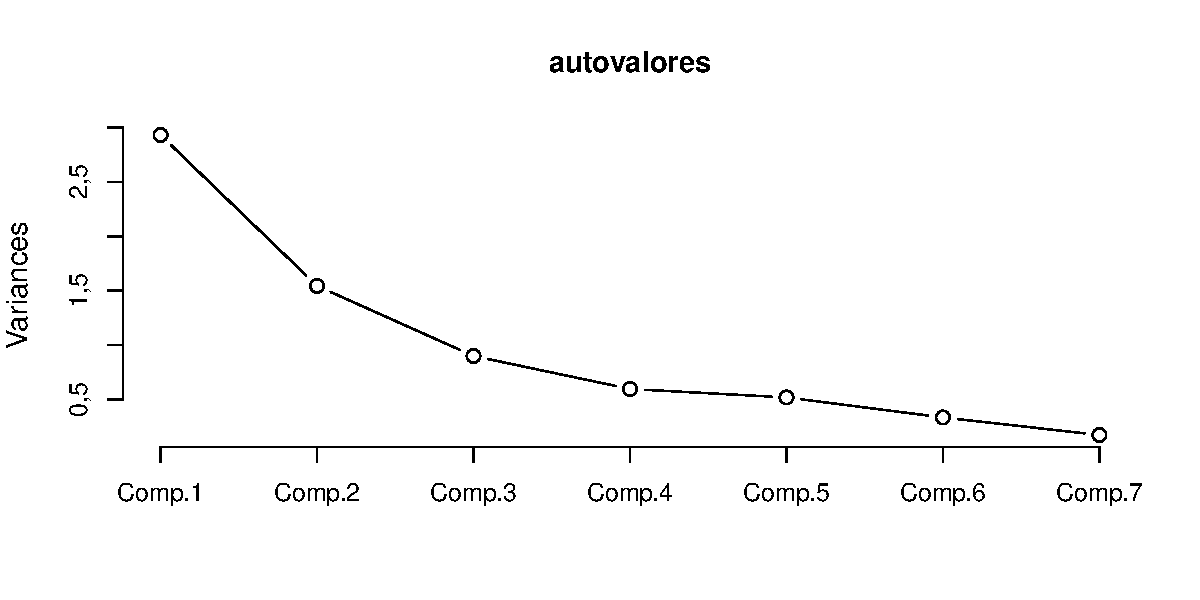
\includegraphics{RELATORIO_FINAL_FORMATADO_files/figure-latex/unnamed-chunk-13-1} 

}

\caption{Quantil-quantil para cada Grupo}\label{fig:unnamed-chunk-13}
\end{figure}

Na Figura 5, podemos ver que a normalidade bivariada não parece ser uma
suposição razoável para nenhum dos grupos, porque além da sistematização
em torno da linha de referência, existem muitos pontos fora das bandas
de confiança. Dadas as observações, vemos que a suposição de normalidade
multivariada para ambas as regiões parece ser irrazoável. Contudo, a
técnica de análise discriminante de Fisher foi desenvolvida sem supor
normalidade dos dados. Assim, a suposição de normalidade avaliadas com
base nos gráficos 4 e 5 não é relevante para a aplicação da técnica de
análise discriminante de Fisher.

\vspace{0.5cm}

\begin{figure}[!h]

{\centering 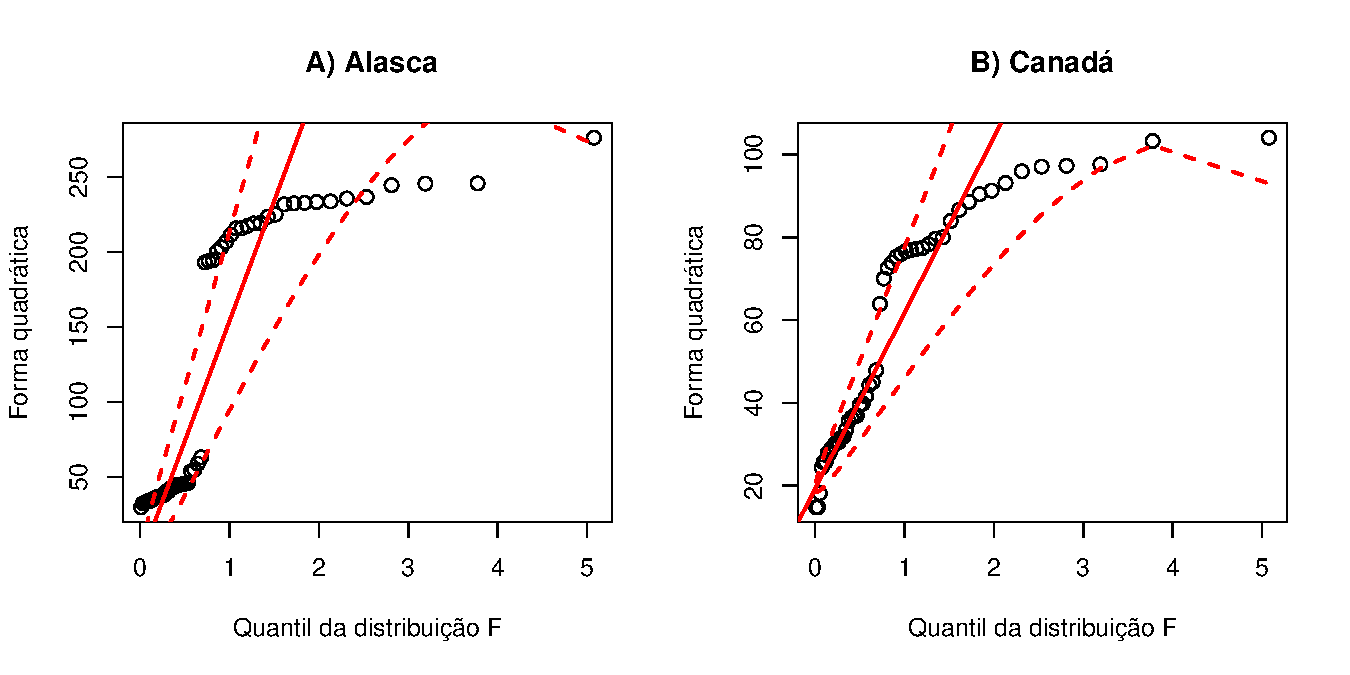
\includegraphics{RELATORIO_FINAL_FORMATADO_files/figure-latex/unnamed-chunk-14-1} 

}

\caption{Gráfico de quantil-quantil com envelopes para a distância de Mahalanobis; A) Alasca, B) Canadá}\label{fig:unnamed-chunk-14}
\end{figure}

\vspace{0.5cm}

Foi realizado o teste de Box para a igualdade de matrizes de
covariâncias dos dados dos tipos de salmão das duas regiões (Alasca e
Canadá), resultando num p-valor = 0,013 e, indicando que existe
diferença estatisticamente significante entre as matrizes de
covariâncias dos tipos de salmão e que não parece ser razoável a
suposição de igualdade das matrizes de covariâncias entre os tipos de
salmão. Este resultado tem grande relevância, uma vez que a técnica de
análise discriminante de Fisher supõe homocedasticidade multivariada, ou
seja, igualdade das matrizes de covariâncias para os grupos. O teste de
box, portanto, indicou que a suposição de homocedasticidade neste caso
não parece ser razoável quando se considera os grupos de salmão
originários do Alasca e do Canadá.

Foi realizado o teste de Box para igualdade de matrizes de covariâncias
dos dados dos dois tipos de salmão macho, ao qual resultou num p-valor
0,013, indicando que existe diferença estatisticamente significante
entre as matrizes de covariâncias dos tipos de salmão machos e que não
parece ser razoável a suposição de igualdade das matrizes de
covariâncias entre os tipos de salmão macho. O teste de Box, portanto,
indicou que a suposição de homocedasticidade neste caso não parece ser
razoável quando se considera os grupos de salmão do sexo masculino
originários do Alasca e do Canadá.

Também foi realizado um teste de Box para igualdade de matrizes de
covariâncias dos dados dos dois tipos de salmão fêmea, ao qual resultou
num p-valor 0,013, indicando que existe diferença estatisticamente
significante entre as matrizes de covariâncias dos tipos de salmão
fêmeas, indicando que não parece ser razoável a suposição de igualdade
das matrizes de covariâncias entre os tipos de salmão femea. O teste de
box, portanto, indicou que a suposição de homocedasticidade neste caso
não parece ser razoável quando se considera os grupos de salmão do sexo
feminino originários do Alasca e do Canadá.

\newpage

\vspace{0.5cm}

\begin{enumerate}
\def\labelenumi{\arabic{enumi}.}
\setcounter{enumi}{2}
\tightlist
\item
  Análise Inferencial
\end{enumerate}

\vspace{0.5cm}

Não encontramos nenhuma informação que nos dê direcionamento direto à
definição de probabilidades a priori de um salmão ser proveniente de uma
ou outra localidade (Alasca ou Canadá), uma vez que essa probabilidade
está muito relacionada ao local onde o salmão foi pescado. Por não ter
informações suficientes iríamos supor probabilidades iguais para cada
localidade. Porém como foi orientado utilizar probabilidades diferentes
para cada localidade, utilizamos os dados sobre toneladas de salmão
comercial pescados e seus respectivos valores monetários gerados no ano
de 2015 (dado mais atual) a partir dessa pesca para as duas localidades
Estes valores são apresentados na Tabela 01 (``tabela com as quantidades
de salmão Alasca/CANADA e \$''). Observamos que o volume de pesca de
salmão para o ano de 2015 é muito maior no Alasca em comparação com o
Canadá. Isso nos leva a acreditar que a população de salmão do Alasca é
maior que a população de salmão do Canadá e que nos leva a conjecturar
que a probabilidade de um salmão ser originário do Alasca é maior do que
um salmão ser originário do Canadá. Acreditamos que considerar a
probabilidade a priori de um salmão ser originário do Alasca como sendo
0,6 e ser originário do Canadá como sendo 0,4 parece ser razoável diante
dos dados da Tabela 1 e da relação levantada entre a probabilidade do
salmão pertencer a uma determinada localidade e o local da pesca, uma
vez que não se tem informações mais precisas quanto às populações de
salmão e seus respectivos comportamentos migratórios destes de ambas as
localidades.

Com base na metodologia de Análise discriminante de Fisher, considerando
custos iguais de classificação errada e probabilidades a priori
destacadas acima, obtivemos uma regra de classificação a qual estão
apresentados os seguintes resultados.

\vspace{0.5cm}

\vspace{0.5cm}

\begin{table}[ht]
\centering
\caption{Resultados da classificação da amostra teste}
\bgroup
\def\arraystretch{1.5}
\begin{tabular}{rrr}
\toprule
& Alasca & Canadá \\ \midrule
\hline
Alasca & 23 & 2 \\
Canadá & 1 & 24 \\ \bottomrule
\hline
\end{tabular}
\egroup
\end{table}

\vspace{0.5cm}

Ao observar a Tabela 3 (Resultados da classificação da amostra teste),
observamos a qualidade da regra de classificação e obtemos uma taxa de
erro aparente TEA = 6 \(\%\), valor bem próximo ao da taxa ótima de erro
TOE = 5,26 \(\%\) ao qual leva em consideração a validade da suposição
de igualdade das matrizes de covariância relativas aos dois tipos de
salmão, ou seja, mesmo com as observações indicativas à fuga da
suposição mencionadas, a regra de classificação mostrou uma taxa de erro
bem próxima à taxa ótima, indicando uma boa performance da regra
proposta.

A Tabela 4 (Medidas resumo para os valores função discriminante aplicada
na amostra teste, por grupo:) apresenta medidas resumo para os valores
da função discriminante e a Figura 6 (Boxplots da função discriminante
aplicada à amostra teste, por grupo) apresenta os boxplots para estes
mesmos valores. Notamos que o valor máximo para o grupo Alasca é bem
próximo ao valor da mediana para o grupo Canadá. O mesmo acontece para o
mínimo do grupo Canadá em comparação com a mediana do grupo Alasca, o
desvio padrão dos valores dos dois grupos é bastante similar (diferença
de 0,19). Para ambos os grupos, os valores da média e mediana se
apresentam com valores bastante próximos e os boxplots parecem ser
simétricos (ou pouco assimétricos).

A Figura 7 (Densidade estimada da função discriminante aplicada à
amostra teste, por grupo)) apresenta as densidades estimadas da função
discriminante para os grupos. À luz do comportamento apresentado pelos
boxplots temos uma interseção entre estas densidades, o que demonstra
que a regra de decisão obtida não consegue isolar totalmente as
distribuições e consequentemente, diferenciar totalmente os tipos de
salmão. Porém isso é intrínseco ao banco de dados, já que as variáveis
propriamente não tem um comportamento totalmente distinto entre os tipos
de salmão.

\vspace{0.5cm}

\begin{table}[ht]
\centering
\caption{Medidas resumo para os valores função discriminante aplicada na amostra teste, por grupo:}
\bgroup
\def\arraystretch{1.5}
\begin{tabular}{rlrrrrrrr}
\toprule
& Grupo & Média & DP & Var. & Mínimo & Mediana & Máximo & n \\ \midrule
\hline
1 & Alasca & -0,63 & 1,15 & 1,33 & -3,16 & -0,62 & 1,94 & 25 \\
2 & Canadá & 1,97 & 0,96 & 0,93 & -0,64 & 1,97 & 3,77 & 25 \\ \bottomrule
\hline
\end{tabular}
\egroup
\end{table}

\vspace{1.0cm}

\begin{figure}[!h]

{\centering 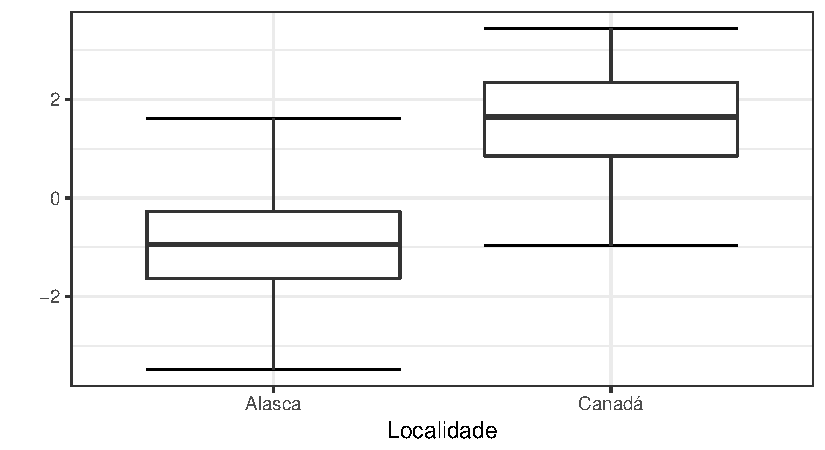
\includegraphics{RELATORIO_FINAL_FORMATADO_files/figure-latex/unnamed-chunk-22-1} 

}

\caption{Boxplots da função discriminante aplicada à amostra teste, por grupo}\label{fig:unnamed-chunk-22}
\end{figure}

\begin{figure}[!h]

{\centering 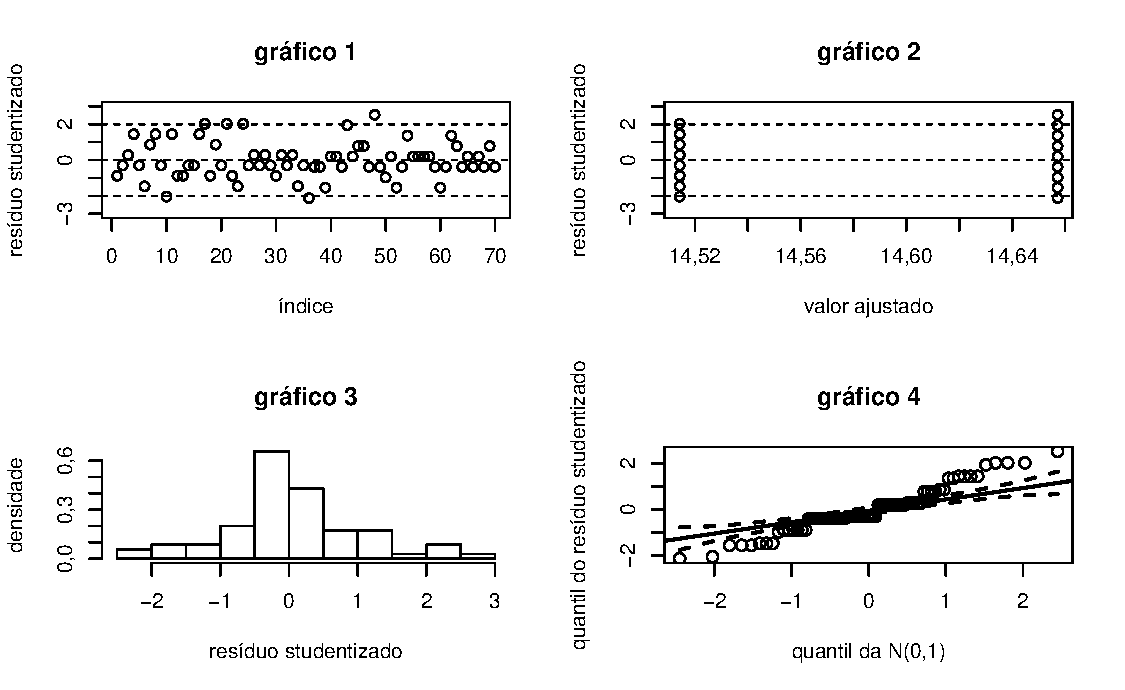
\includegraphics{RELATORIO_FINAL_FORMATADO_files/figure-latex/unnamed-chunk-23-1} 

}

\caption{Densidade estimada da função discriminante aplicada à amostra teste, por grupo}\label{fig:unnamed-chunk-23}
\end{figure}

\newpage

\begin{center}
\textbf{Análise considerando a variável gênero}
\end{center}

\begin{enumerate}
\def\labelenumi{\arabic{enumi}.}
\setcounter{enumi}{3}
\tightlist
\item
  Análise Descritiva
\end{enumerate}

\begin{table}[!h]
\centering
\caption{Medidas Resumo das variáveis por região, considerando a variável gênero}
\bgroup
\def\arraystretch{1.5}
\begin{tabular}{rlllllllll}
  \toprule
 & Gênero & n & Media & Variancia & Desvio Padrao & CV(\%) & Minimo & Mediana & Maximo \\ \midrule
  \hline
1 & Fêmea & 52 & 118,058 & 777,114 & 27,877 & 23,613 & 53 & 118,5 & 179 \\ 
  2 & Macho & 48 & 117,771 & 580,734 & 24,098 & 20,462 & 79 & 117 & 170 \\ \midrule
  3 & Fêmea & 52 & 396,327 & 1808,773 & 42,53 & 10,731 & 301 & 397,5 & 481 \\ 
  4 & Macho & 48 & 400,104 & 2533,457 & 50,333 & 12,58 & 306 & 388,5 & 511 \\ \bottomrule
   \hline
\end{tabular}
\egroup
\end{table}

A partir da Figura 9, que consta o gráfico de dispersão entre as
variaveis separadas por Região (Alasca e Canadá). Para o gênero Fêmea,
podemos observar que os peixes do Canáda tendem a ter um diâmetro (em
mm) da guelra durante a fase de água doce maior que os indivíduos do
Alasca e durante a fase no Mar tendem a ter um diametro menor (em mm).
Se olharmos separadamente os dois grupos, vemos que existe uma
correlação levemente positiva de valor 0,22 entre os indivíduos do
Canadá, e levemente negativa de valor -0,35 para os índividuos do
Alasca. Vale ressaltar que se considerarmos ambos os Grupos, parecer
haver uma correlação levemente negativa entre as variaveis. O mesmo é
observado para o grupo dos machos,se olharmos separadamente os dois
grupos, vemos que existe uma correlação levemente positiva de valor 0,27
entre os indivíduos do Canadá, e levemente negativa de valor -0,36 para
os índividuos do Alasca.

\begin{figure}[!h]

{\centering 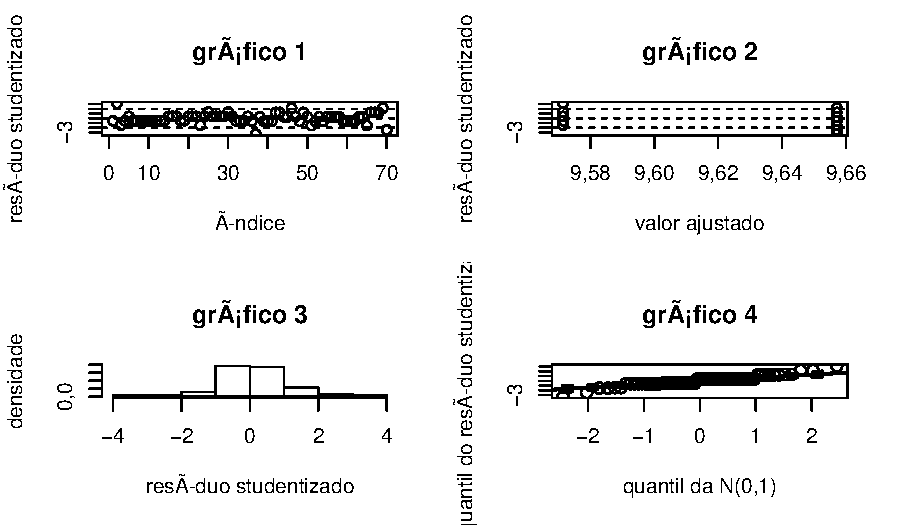
\includegraphics{RELATORIO_FINAL_FORMATADO_files/figure-latex/unnamed-chunk-31-1} 

}

\caption{ Gráfico de dispersão entre os diâmetros da guelra de salmões em água doce e no mar - Macho}\label{fig:unnamed-chunk-31}
\end{figure}

\vspace{0.5cm}

\begin{figure}[!h]

{\centering 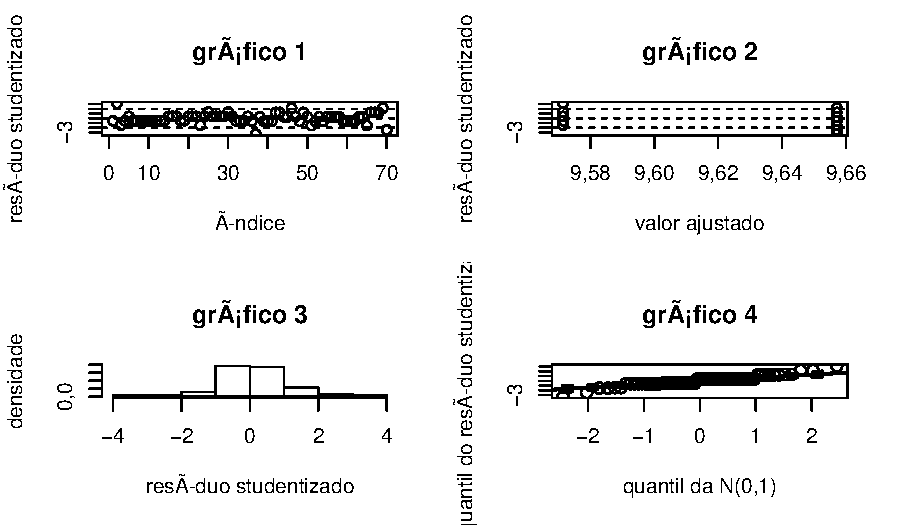
\includegraphics{RELATORIO_FINAL_FORMATADO_files/figure-latex/unnamed-chunk-32-1} 

}

\caption{Gráfico de dispersão entre os diâmetros da guelra de salmões em água doce e no mar- Fêmea}\label{fig:unnamed-chunk-32}
\end{figure}

A partir dos Box-plot da Figura 10, podemos ver para o gênero macho que
o diâmetro das guelras do Canadá na fase em agua doce consideravelmente
maior que o Grupo Alasca, já para a Fase no mar o contrario ocorre.

Além disso podemos ver que o diâmetro das guelras para o salmão fêmea do
Canadá é consideravelmente maior do que os do Alasca, já durante a fase
no mar, o contrario ocorre e para o Canadá o valor máximo quase atinge a
mediana do grupo Alasca.

Portanto é possível notar a partir dos densidades é possível notar que
existe uma sobreposição em boa parte da distribuições apresentadas, o
que já foi notado nos boxplots anteriormente.

\begin{figure}[!h]

{\centering 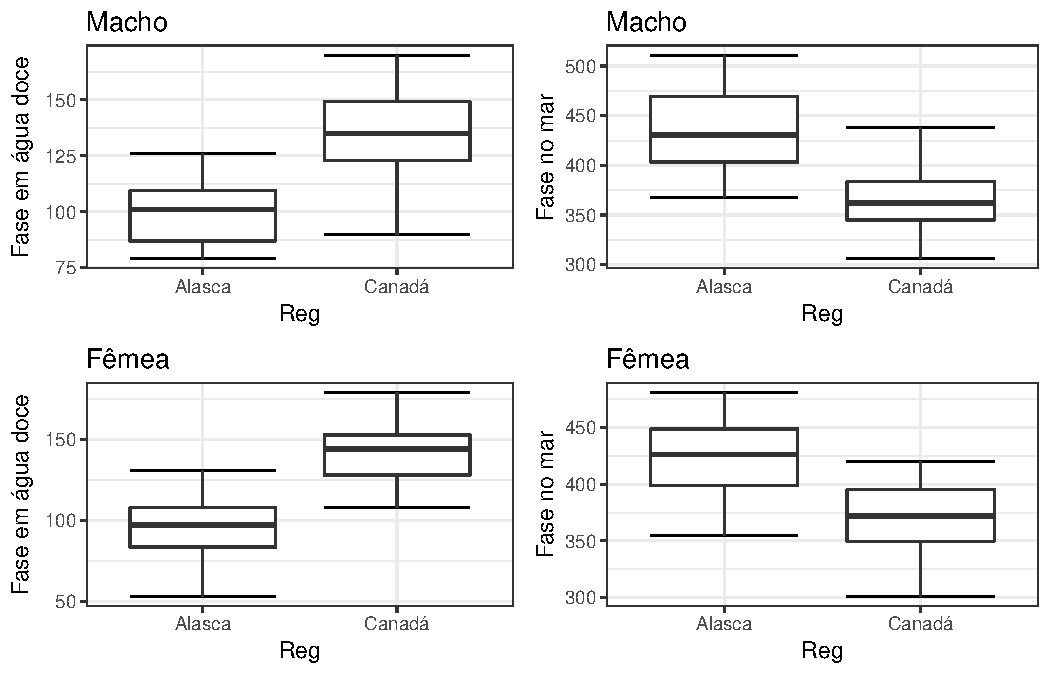
\includegraphics{RELATORIO_FINAL_FORMATADO_files/figure-latex/unnamed-chunk-33-1} 

}

\caption{Boxplots dos Grupos por Gênero}\label{fig:unnamed-chunk-33}
\end{figure}

\vspace{0.5cm}

\begin{figure}[!h]

{\centering 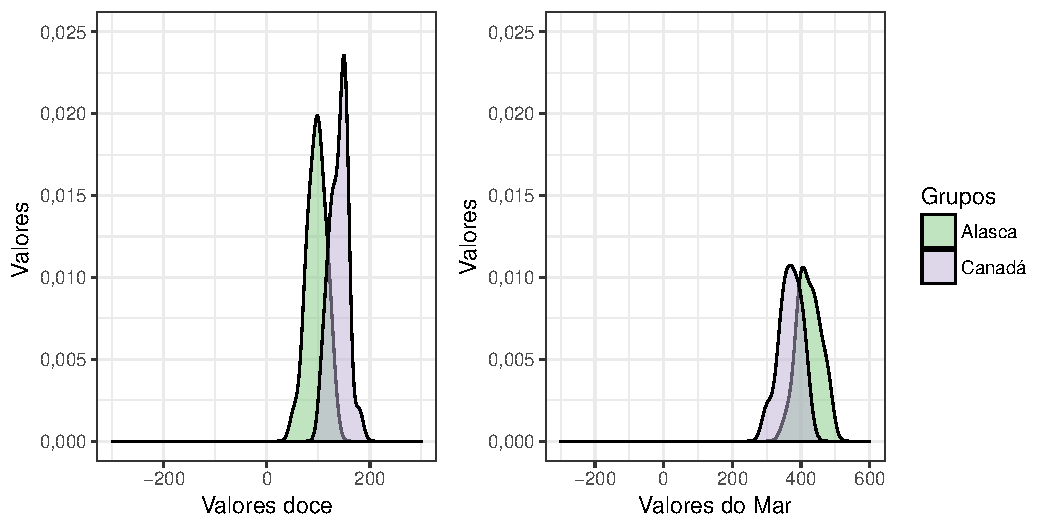
\includegraphics{RELATORIO_FINAL_FORMATADO_files/figure-latex/unnamed-chunk-34-1} 

}

\caption{Densidades dos grupos do gênero -  Fêmea}\label{fig:unnamed-chunk-34}
\end{figure}

\vspace{0.5cm}

\begin{figure}[!h]

{\centering 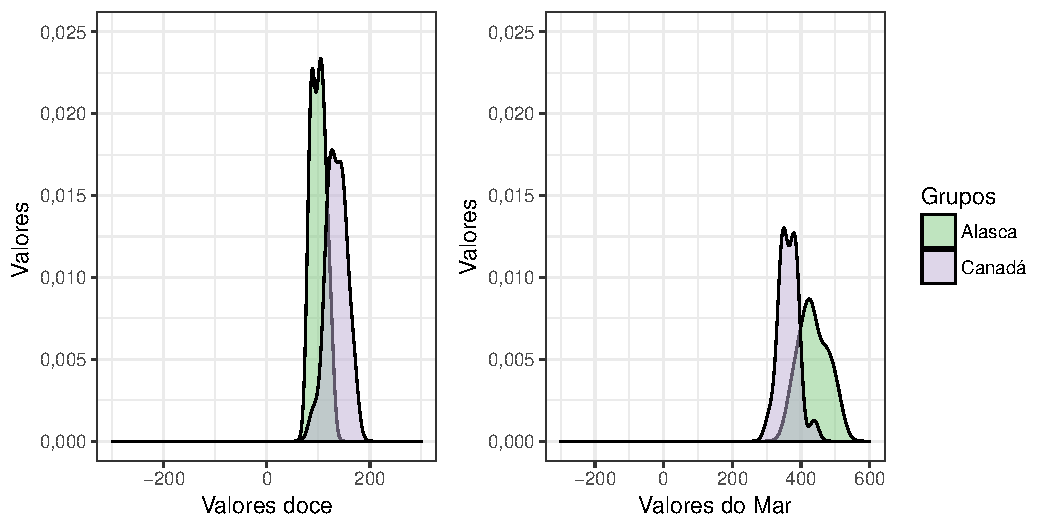
\includegraphics{RELATORIO_FINAL_FORMATADO_files/figure-latex/unnamed-chunk-35-1} 

}

\caption{Densidades dos grupos do gênero -  Macho}\label{fig:unnamed-chunk-35}
\end{figure}

\vspace{0.5cm}

\newpage

\begin{enumerate}
\def\labelenumi{\arabic{enumi}.}
\setcounter{enumi}{4}
\tightlist
\item
  Análise Inferencial
\end{enumerate}

\vspace{0.5cm} Outras duas regras, baseadas na metodologia de Análise
discriminante de Fisher, foram geradas a partir do banco de dados. Porém
agora os grupos (Alasca e Canadá) foram divididos por sexo fêmea e
macho. Aqui também foi suposto a presença de homocedasticidade entre as
populações, com custos de classificação errada iguais e com as mesmas
prioris definidas anteriormente, ou seja, as probabilidades a priori de
um salmão pertencer ao Grupo Alasca foi definida como 0,6 e pertencer ao
grupo Canadá foi 0,4 para ambos os sexos.

Como já foi discutido anteriormente, o teste de Box indicou para ambos
os sexos que as matrizes de covariância são diferentes, de modo que a
suposição de homocedasticidade não parece ser razoável para ambos os
casos.

Os resultados referentes às regras de classificação para salmões fêmea e
macho são apresentados na tabela 5.

\begin{table}[!h]
\centering
\caption{Resultados da classificação da amostra teste}
\bgroup
\def\arraystretch{1.5}
\begin{tabular}{llll} \toprule
                       &           & \multicolumn{2}{l}{Classificado} \\
\cline{3-4}
                       & Observado & Alasca        & Canadá         \\ \midrule
\multirow{2}{*}{Fêmea} & Alasca    &      12        &     1           \\
                       & Canadá    &       0        &     13          \\ \midrule
\multirow{2}{*}{Macho} & Alasca    &      12        &     0           \\
                       & Canadá    &      1         &     11         \\ \bottomrule
   \hline
\end{tabular}
\egroup
\end{table}

Ao observar a Tabela 5, observamos a qualidade da regra de classificação
para os salmões fêmea. Obtivemos uma taxa de erro aparente TEA = 0,04
\(\%\), valor bem abaixo ao da taxa ótima de erro TOE = 0,07 \(\%\) ao
qual leva em consideração a validade das suposições de igualdade das
matrizes de covariância relativas aos dois tipos de salmão, ou seja,
mesmo com as observações indicativas à fuga da suposição mencionadas, a
regra de classificação mostrou uma taxa de erro ainda menor que a taxa
ótima, indicando uma boa performance da regra proposta para o banco de
dados em questão.

TEA(Feminino): 0,0384615

TOE(Feminino): 0,0658768

Para os machos, observamos a qualidade da regra de classificação para os
salmões macho. OBtivemos uma taxa de erro aparente TEA = 0 \(\%\), valor
bem abaixo ao da taxa ótima de erro TOE = 0,13 \(\%\) ao qual leva em
consideração a validade das suposição de igualdade das matrizes de
covariância relativas aos dois tipos de salmão, ou seja, mesmo com as
observações indicativas a fuga da suposição mencionadas, a regra de
classificação mostrou uma taxa de erro ainda menor que a taxa ótima,
indicando uma boa performance da regra proposta para o banco de dados em
questão.

TEA(Masculino): 0

TOE(Masculino): 0,128419

Observamos também que as regras de classificação para os salmões fêmea e
macho apresentam valores de TEA bastante similares, já que ambos tiveram
apenas um erro de classificação e a quantidade de peixes de cada sexo na
amostra onde as regras foram testadas é praticamente a mesma.

Na tabela 7 podemos verificar as medidas resumos dos grupos divididos
por macho e fêmea, onde são apresentadas os valores da função
discriminante aplicada na amostra teste. Além disso é possível observar
os box-plots para cada sexo na figura 13 (boxplot fêmea).

Para salmões fêmea, observamos que o valor mínimo referente ao grupo
Canadá é menor que o máximo referente ao grupo Alasca, porém, pode-se
observar por meio dos box-plots correspondentes que a menos de alguns
valores discrepante, os box-plots parecem ser bastante distintos, uma
vez que, pode-se perceber uma separação clara entre valores presentes no
grupo Alasca, se comparados com os valores presentes no grupo Canadá.
Este comportamento também é observado, embora seja menos evidente, na
figura XX (função discriminante fêmea) ao qual apresenta as densidades
estimadas para os valores da função discriminante para os grupos. Nesta
figura observa-se uma área de interseção pequena entre as densidades, o
que favorece a distinção da origem dos almões fêmea por meio das
variáveis DGAD e DGM.

O comportamento referente aos valores da função discriminante para
salmões macho é análogo ao apresentado para salmões fêmea. Os box-plots
correspondentes, a menos de dois pontos, parecem ser bastante distintos,
assim como existe pouca área de interseção entre as densidades estimadas
para os valores da função discriminante para os grupos Alasca e Canadá
(Figura XX ((funçao discriminante macho)), o que favorece a distinção da
origem dos salmões macho por meio das variáveis DGAD e DGM.

\begin{table}[!h]
\centering
\caption{Medidas resumo para os valores função discriminante aplicada na amostra teste considerando a variável gênero}
\begin{tabular}{llrrrrrrr}
\hline
Gênero & Localidade & Média & DP & Var. & Mínimo & Mediana & Máximo & n \\
\hline
\hline
\multirow{2}{*}{Fêmea}& Alasca & -1,18 & 1,11 & 1,23 & -2,39 & -1,44 & 1,49 & 13 \\
& Canadá & 1,80 & 0,79 & 0,62 & -0,71 & 1,80 & 3,26 & 13 \\
\hline
\multirow{2}{*}{Macho}& Alasca & -1,50 & 0,87 & 0,76 & -3,23 & -1,68 & 0,26 & 12 \\
& Canadá & 1,53 & 0,95 & 0,90 & -0,80 & -1,81 & 2,58 & 12 \\
\hline
\end{tabular}
\end{table}

\vspace{1.5cm}

\begin{figure}[!h]

{\centering 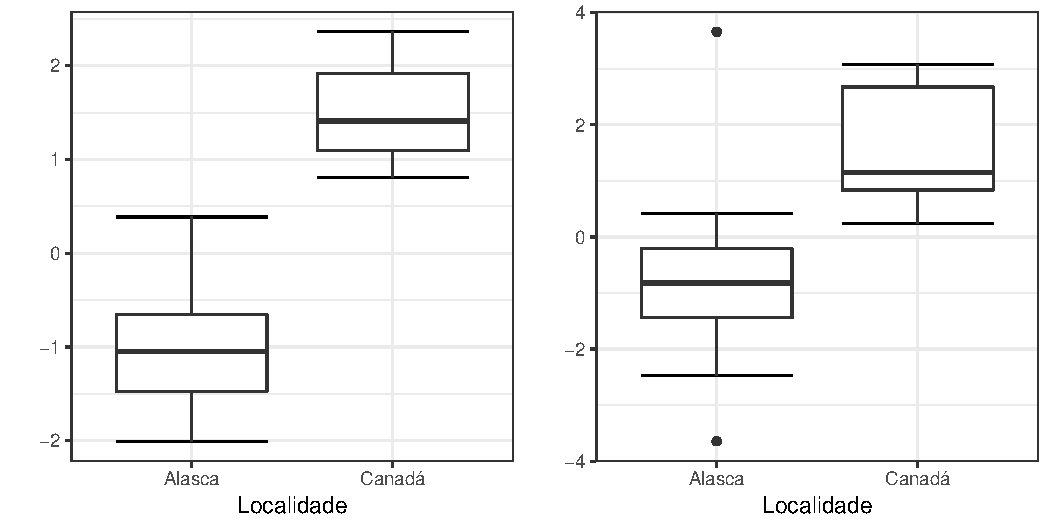
\includegraphics{RELATORIO_FINAL_FORMATADO_files/figure-latex/unnamed-chunk-40-1} 

}

\caption{Boxplots da função discriminante aplicada à amostra teste, por grupo}\label{fig:unnamed-chunk-40}
\end{figure}

\begin{figure}[!h]

{\centering 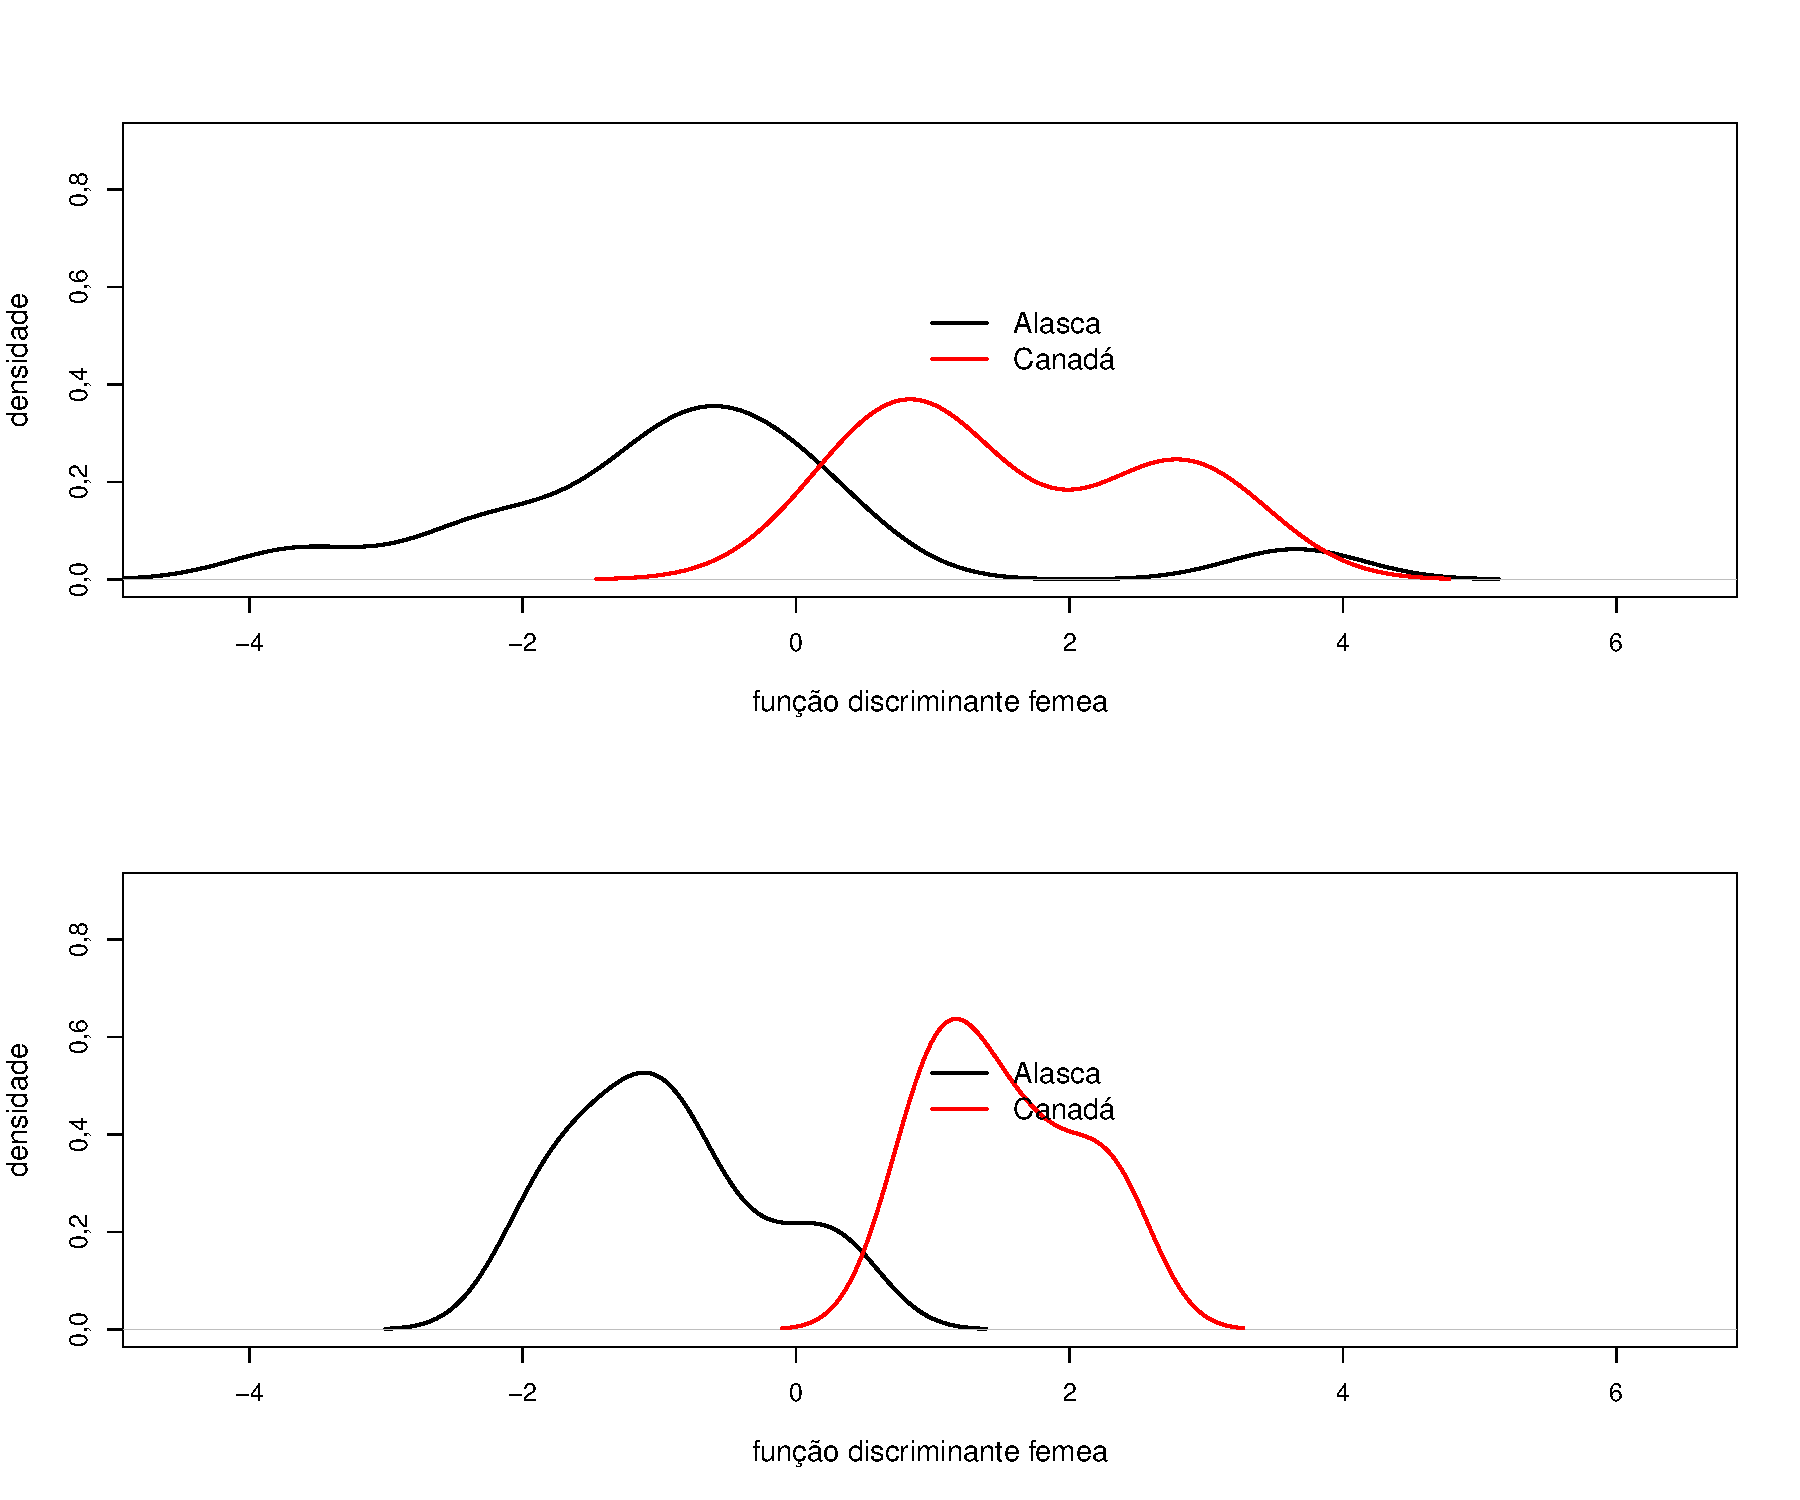
\includegraphics{RELATORIO_FINAL_FORMATADO_files/figure-latex/unnamed-chunk-41-1} 

}

\caption{Densidade estimada da função discriminante aplicada à amostra teste, por grupo}\label{fig:unnamed-chunk-41}
\end{figure}

\newpage

\vspace{0.5cm} 6.Conclusões

\vspace{0.5cm}

As análises apresentadas aqui indicaram que as regras de classificação
de salmões quanto à sua origem (Alasca ou Canadá) obtidas por meio do
método de análise discriminante de Fisher foram razoavelmente boas,
mesmo sendo a suposição de homocedasticidade irrazoável para todos os
conjuntos analisados (Salmões de ambos os sexos, Salmões macho e Salmões
fêmea).

Concluimos que todas as regras de classificação obtidas neste presente
estudo poderiam ser sugeridas, embora as regras obtidas separando-se os
salmões por sexo tenham sido um pouco mais efetivas, errando a
classificação de 2 salmões em contrapartida aos 3 erros de classificação
obtidos pela regra que não leva em consideração os sexos dos peixes para
a mesma quantidade de peixes analisados. Porém deve-se avaliar sempre o
contexto no qual a regra será aplicada, o custo, a utilidade e a
influência que esta regra de classificação pode exercer.

\vspace{0.5cm} 7. Bibliografia \vspace{0.5cm}

\begin{enumerate}
  \item THE PACIFIC SALMON TREATY: A BRIEF TRUCE IN THE CANADA/U.S.A. PACIFIC SALMON WAR.

  \item note="\url{http://www.adfg.alaska.gov/index.cfm?adfg=commercialbyfisherysalmon.salmon_combined_historical}"

  \item note="\url{http://www.pac.dfo-mpo.gc.ca/stats/comm/summ-somm/annsumm-sommann/2015/ANNUAL15_USER_three_party_groups-eng.htm}"

  \item Azevedo, C. L. N. (2017). Notas de aula sobre análise multivariada de dados note= "\url{http://www.ime.unicamp.br/~cnaber/Material_AM_2S_2017.htm}" 

  \item Johnson, R. A. e Wichern, D. W. (2007). Applied Multivariate Statistical Analysis. 6 a edição, Upper Saddle River, NJ: Pearson Prentice Hall.
  
\end{enumerate}


\end{document}
